\chapter{\IfLanguageName{dutch}{Stand van zaken}{State of the art}}
\label{ch:stand-van-zaken}

% Tip: Begin elk hoofdstuk met een paragraaf inleiding die beschrijft hoe
% dit hoofdstuk past binnen het geheel van de bachelorproef. Geef in het
% bijzonder aan wat de link is met het vorige en volgende hoofdstuk.

% Pas na deze inleidende paragraaf komt de eerste sectiehoofding.


\section{Angular}

Angular is een framework dat het gemakkelijk maakt om webapplicaties te bouwen. Angular combineert templates, dependency injectie, end to end tooling en geïntegreerde best practices om hindernissen in de ontwikkeling op te lossen. Angular stelt ontwikkelaars in staat om applicaties te maken voor op het web, mobiel of desktop. \autocite{Lotanna2019}

Angular kan gezien worden als een volwaardig MVC\footnote{Model View Controller} framework. Het wordt zo beschouwd omdat Angular de structuur van de applicatie in ontwikkeling sterk wil regulieren. Angular voorziet standaard veel functionaliteit. Aan de andere kant zorgt dit wel voor minder flexibiliteit. Angular verstrekt onderstaande functionaliteit. \autocite{Hamedani2018}
\begin{itemize}
	\item Templates
	\item XSS\footnote{Cross-Site Scripting} bescherming
	\item Dependency Injectie
	\item Component CSS encapsulatie
	\item Hulpmiddelen voor het unit-testen van componenten
	\item Ajax requests
	\item Routering
	\item Formulieren
\end{itemize}

Google, de ontwikkelaar van AngularJS, kondigde eind 2014 aan dat Angular 2 een volledige herschrijving van AngularJS zou zijn. Ze zouden zelf een nieuwe programmeertaal \texttt{AtScript} ontwikkelen die speciaal voor Angular 2 bedoeld was. Toen begon Microsoft decorators te ondersteunen in hun taal TypeScript, waardoor deze de aanbevolen taal werd voor de ontwikkeling van Angular 2 applicaties. Het is echter ook mogelijk om applicaties te ontwikkelen in JavaScript (ECMAScript 5 en ECMAScript 6) en in Dart. \autocite{Fain2016}

% explain AngularJS
% explain decorator
% explain typescript (strict superset etc.)
% explain dart

Het team van Google besliste om geen grote updates meer te doen aan AngularJS omdat ze, naast het verbeteren van features en prestaties, Angular meer future-proof wilden maken door gebruik te maken van web componenten en ECMAScript 6. Het resultaat was Angular 2, verrijkt met enorm veel features. De voornaamste nieuwe features waren niet mogelijk in AngularJS waardoor een herschrijving nodig was. Als eerste was de ideologie veranderd. Bij AngularJS lag de focus op databinding en templates. Het belangrijkste doel was om af te komen van het traditionele proces voor DOM-handling via JavaScript's jQuery. Daarnaast moest het framework ook klaar voor de toekomst zijn. Sinds de meeste browsers ECMAScript 6 gebruiken, zullen applicaties dus ook ontwikkeld moeten worden in ES6. Angular 2 biedt die kans aan, met 100\% browser achterwaartse compatibiliteit. Ook maakt Angular 2 gebruik van web componenten. Dit zijn JavaScript en HTML modules die gemaakt worden voor een specifieke taak in de applicatie. Als laatste werden routers, dependency injection, dynamic loading en async templating verbeterd of toegevoegd. Angular 2 werd uitgegeven in 2016. \autocite{Shan2015}

% explain databinding
% explain backward compat
% explain web components?
% explain jquery
% explain routers, di, dynamic loading, async templating

\subsection{Inleiding}
%https://angular.io/guide/architecture

De basis-bouwstenen van Angular applicaties zijn NgModules. Deze voorzien compilatie context voor componenten en verzamelen gerelateerde code in functionele sets. Een Angular applicatie wordt bepaald door een set van NgModules. Elke applicatie heeft een root module dat bootstrapping mogelijk maakt. Daarnaast kunnen nog meerdere feature modules toegevoegd worden, maar deze zijn niet verplicht. \autocite{Angular2019a}

Componenten definiëren views, dit zijn sets van schermelementen die Angular kan gebruiken en aanpassen aan de hand van de logica in de applicatie. Daarnaast kunnen componenten services gebruiken die specifieke functionaliteiten voorziet die niet verbonden zijn met views. Deze services kunnen geïnjecteerd worden in componenten met behulp van dependency injection. Hierdoor wordt de code herbruikbaar en modulair. \autocite{Angular2019a}
% explain modulair?

Zowel componenten als services zijn gewone klassen met decorators. Deze kenmerken hun type en voorzien metadata. Angular gebruikt deze metadata om te weten hoe deze klassen gebruikt kunnen worden. De metadata van een component verbindt de component met een template die een view definieert. Een template combineert HTML met Angular directives en binding markup die Angular toestaan om de HTML aan te passen voordat het getoond wordt op het scherm. Daarnaast voorziet de metadata van een service de informatie die Angular nodig heeft om het beschikbaar te maken voor componenten via dependency injection. \autocite{Angular2019a}
% verklarende lijst: dependency injection (DI)

\subsection{Modules}
%https://angular.io/guide/architecture-modules

Angular applicaties zijn \texttt{modulair}. NgModules zijn containers die samenhangende code van een bepaald domein of bepaalde workflow bevat. Ze kunnen componenten, services en andere code-bestanden die behoren tot de scope van de module bevatten. Ook kan functionaliteit geïmporteerd worden van een andere NgModule. Daarnaast kan een NgModule bepaalde functionaliteiten exporteren die andere NgModules kunnen gebruiken. Elke applicatie heeft minstens een NgModule klasse, de root module. Deze heet gewoonlijk AppModule en bevind zich in een bestand genaamd \texttt{app.module.ts}. De applicatie wordt gestart door deze root module te bootstrappen. Zoals eerder vermeld kunnen dus extra modules toegevoegd worden als feature modules. De AppModule kan deze extra modules omvatten in een hiërarchie met onbepaalde diepte. \autocite{Angular2019b}

Een NgModule wordt gedefinieerd door een klasse met de \texttt{@NgModule()} decorator. Deze decorator is een functie die een metadata object verwacht. De properties van dit object worden omschreven in de module. Enkele van de belangrijkste properties van een module zijn als volgt \autocite{Angular2019b}:
\begin{itemize}
    \item Declarations: set van componenten, directives en pipes die tot de module behoren.
    \item Exports: set van declarations die zichtbaar en bruikbaar moeten zijn in component templates van andere modules.
    \item Imports: set van modules die nodig zijn in component templates die gedefinieerd zijn in de huidige module.
    \item Providers: set van services (meer uitleg hier)
    \item Bootstrap: Dit is de view van de main applicatie, genaamd de root component. Deze host alle andere views van de applicatie. Dit kan enkel voor de root NgModule. 
\end{itemize}


% simpele root NgModule declaratie
% insert image van https://angular.io/guide/architecture-modules
% simpele normale NgModule declaratie
% insert image

Modules voorzien compilatie context voor de componenten die ze declareren. De root module heeft altijd een root component die aangemaakt wordt tijdens de bootstrap. Elke module kan extra componenten omvatten die met behulp van de router geladen kunnen worden of aangemaakt kunnen worden door de template. \autocite{Angular2019b} 

% misschien bij view?
Een view wordt gedefinieerd door een component en zijn template. Een component kan een view hiërarchie bevatten die toestaat om een complexe samenstelling van een scherm te definiëren. Deze samenstelling kan als een eenheid aangemaakt, aangepast en verwijderd worden. De hiërarchie bestaat uit een enkele host view. Deze view kan de root van een hiërarchie zijn die \texttt{embedded views} kan bevatten, die op hun beurt host view zijn van een andere component. Deze componenten kunnen deel zijn van dezelfde module of geïmporteerd worden van een andere module. \autocite{Angular2019b}
% explain embedded
% insert image van https://angular.io/guide/architecture-modules

De NgModules van Angular zijn totaal verschillend van de JavaScript modules. In JavaScript is elk bestand een module en elk object gedefinieerd in dat bestand behoort tot die module. Die objecten kunnen geëxporteerd worden door de module door gebruik te maken van het sleutelwoord \texttt{export}. Andere modules kunnen dan gebruik maken van dit publiek object door het sleutelwoord \texttt{import} te gebruiken. \autocite{Angular2019b}

\subsection{Componenten}
%https://angular.io/guide/architecture

Elke applicatie heeft naast een module ook minstens een component, de root component. Die legt de verbinding tussen een component's view hiërarchie en het DOM. Elke component definieert een klasse die applicatiedata en -logica bevat. Deze wordt ook verbonden met een HTML-template die een view definieert. De \texttt{@Component()} decorator identificieert de onderstaande klasse als een component en voorziet de template en alle specifieke metadata voor die component. Deze metadata is net zoals bij NgModules een functie die een object verwacht.  \autocite{Angular2019a}

Een component is dus de meest basis bouwsteen van een Angular applicatie. Zo'n applicatie bestaat meestal uit een \texttt{tree} van Angular componenten. Componenten zijn een subset van \texttt{directives} die altijd geassocieerd worden met een template. Echter in tegenstelling tot \texttt{directives} kan slechts een component geïnstantieerd worden per template-element. Daarnaast kan het gedrag van een component tijdens runtime ook geprogrammeerd worden door gebruik te maken van \texttt{lifecycle hooks} \autocite{Angular2019c}

De voornaamste properties van het metadata-object voor componenten zijn als volgt \autocite{Angular2019c}
\begin{itemize}
    \item ChangeDetection: De change-detection strategie voor de component. Wanneer een component geïnstantieerd wordt, maakt Angular een change detector aan die verantwoordelijk is voor het uitdragen van de bindingen van de component. Er zijn 2 mogelijkheden nl. ChangeDetection\#OnPush: CheckOnce(on demand) en ChangeDetection\#Default: CheckAlways
    \item ViewProviders: definieert een set van injecteerbare objecten die zichtbaar zijn voor de DOM kinderen van de component's view.
    \item Template: Een inline template voor een Angular component.
    \item TemplateUrl: Het relatieve of absolute pad naar een template bestand voor een Angular component. % niet samen met template en vice versa
    \item Styles: Een of meerdere inline CSS stylesheets die gebruikt kunnen worden in de component
    \item StyleUrls: Een of meerdere relatieve of absolute paden naar bestanden die een CSS stylesheet bevatten om te gebruiken in de component. % niet samen met styles en vice versa
    \item EntryComponents: een set van componenten die samen gecompileerd moeten worden met de component. Voor elke component hier gedefinieerd creëert Angular een \texttt{ComponentFactory} en slaat deze op in de \texttt{ComponentFactoryResolver}
    % explain ComponentFactory(Resolver)
\end{itemize}
Daarnaast erft het ook volgende properties over van de \texttt{@Directive()} decorator \autocite{Angular2019c}
\begin{itemize}
    \item Selector: de CSS selector dat de directive identificieert in een template en de instantiatie van de directive start.
    \item Inputs: set van gegevensgebonden properties van de directive.
    \item Outputs: set van eventgebonden properties.
    \item Providers: configureert de injector van de directive met een token dat gemapt wordt naar een provider van een dependency %meer uitleg?
\end{itemize} 

Angular componenten zijn een subset van directives die altijd verbonden zijn met een template. Anders dan andere directives kan maar een component geïnstantieerd worden per element in een template. Een component moet tot een NgModule behoren zodat die beschikbaar zou zijn voor andere componenten. \autocite{Angular2019a}

Een template combineert HTML met Angular markup die HTML-elementen kan aanpassen nog voordat deze getoond worden op het scherm. \autocite{Angular2019a}

Template directives voorzien logica en binding markup verbindt applicatie data met het DOM. Er zijn twee soorten data bindingen. \autocite{Angular2019a}
\begin{itemize}
	\item \texttt{Event binding} staat toe om de applicatie te laten reageren op gebruikers invoer in de omgeving door het aanpassen van applicatie data.
	\item \texttt{Property binding} staat toe om berekende waarden uit de applicatie uit te schrijven in de HTML.
\end{itemize}
Voordat een view getoond wordt op een scherm zal Angular eerst de directives evalueren en de syntax van de binding in de template uitzoeken zodat de HTML elementen en het DOM aangepast kunnen worden, afhankelijk van de applicatie data en logica. Angular staat ook \texttt{two-way-binding} toe. Dit wil zeggen dat zowel aanpassingen in het DOM zoals gebruikers invoer de applicatie data aanpassen en applicatieberekeningen ook weergegeven zullen worden in de HTML. \autocite{Angular2019a}

Een template kan gebruik maken van \texttt{pipes} om de UX\footnote{User Experience: het gevoel en de ervaring dat een gebruiker opdoet} te verbeteren door waarden te transformeren voor weergave. Angular voorziet enkele voorgedefinieerde pipes voor standaard transformaties, maar pipes kunnen ook zelf gedefinieerd worden met een eigen transformatie. \autocite{Angular2019a}
% insert image voorbeeld pipe voor dates

\subsection{Services en DI}
% https://angular.io/guide/architecture

Voor data of logica die niet tot een specifieke view behoort en over de hele applicatie voorzien moet worden, kan een service klasse gebruikt worden. Een service wordt gedefinieerd met de \texttt{@Injecatble()} decorator. \autocite{Angular2019a}

Deze decorator voorziet de metadata die de klasse beschikbaar maakt voor creatie aan een \texttt{Injector} zodat deze geïnjecteerd kan worden als een dependency. Voor elke dependency moet een provider voorzien worden zodat de injector van deze provider gebruik kan maken om een dependency op te halen of een nieuwe aan te maken. Voor een service is dit standaard de service klasse zelf. Angular creëert een globale injector tijdens het bootstrap proces die gebruikt kan worden over de hele applicatie. Daarnaast kunnen extra injectors aangemaakt worden wanneer dat nodig is. \autocite{Angular2019d}

Dependency Injection (DI) is een belangrijk applicatie design pattern. Angular bevat een eigen DI framework dat kenmerkend gebruikt wordt in het design van Angular applicaties om op een efficiënte en modulaire manier om te gaan met het creëren van klassen. Een klasse verzoekt dependencies aan een externe bronnen in plaats van deze zelf aan te maken. In Angular voorziet het DI framework de dependencies aan een klasse zodra deze geïnstantieerd is. \autocite{Angular2019e}
% explain dependencies (services of objecten die een klasse nodig heeft om te kunnen werken.)

Services die aangemaakt worden via het Angular CLI commando \texttt{ng generate service [servicenaam]} registreert een provider voor de service in de root injector door \texttt{'root'} toe te kennen aan het \texttt{providedIn} property van het metadata object. Angular creëert dan een enkele instantie die geïnjecteerd wordt in elke klasse die daar om vraagt. Het \texttt{providedIn} property kan ook een specifiek type zijn. Hierdoor kan Angular de applicatie optimaliseren door de service te verwijderen uit de gecompileerde app wanneer dat type niet gebruikt wordt. Services kunnen ook geregistreerd worden in een specifieke NgModule. De service zal dan beschikbaar zijn voor alle componenten van die module. Om dit te bekomen, moet de service aan de \texttt{providers} set in de module toegevoegd worden. Als laatste kan een provider voor een service ook op component level geregistreerd worden. Op deze manier wordt een nieuwe instantie van de service gemaakt bij elke nieuwe instantie van de component. Dit kan door deze toe te voegen aan de \texttt{providers} property van het metadata object van de component. \autocite{Angular2019d}

Een component kan gebruik maken van een service of andere dependencies door deze te injecteren in de component met behulp van de \texttt{Injector}. Angular creëert alle injectors zelf, dus er moeten geen injectors aangemaakt of geïmplementeerd worden. Een injector maakt de dependencies aan en houdt een container van deze instanties bij zodat deze hergebruikt kunnen worden als dat mogelijk is. Op deze manier krijgt de component toegang tot de service of kan deze de dependency gebruiken. \autocite{Angular2019d}

Wanneer een nieuwe instantie van een component aangemaakt wordt, bepaalt Angular welke dependencies de component nodig heeft door te kijken naar de types van de parameters in de constructor. Dan checkt de injector de container met bestaande instanties. Als deze de gevraagde instantie vindt, wordt die teruggegeven. Indien dat niet het geval is, wordt een nieuwe instantie aangemaakt van de dependency en wordt deze opgeslagen in de container en teruggegeven. \autocite{REFERENCE}
% insert image ??

\subsection{Samenwerking}

Al deze items vormen de basis over de hoofdzakelijke bouwstenen van een Angular applicatie. De afbeelding xx toont hoe deze bouwstenen met elkaar verbonden zijn en samenwerken. 
% insert image whats next
% link naar afbeelding

Een component en een template vormen samen een Angular view. Een \texttt{@Component()} decorator voegt de metadata toe, waarbij een pointer zit naar de geassocieerde template. Directives en binding markup in een template kunnen de view aanpassen afhankelijk van applicatie data en logica. De dependency injector kan services in een component voorzien. Afhankelijk van de provider van de service wordt deze opnieuw aangemaakt. \autocite{Angular2019a}



\section{React}

React, aan de andere kant, is een bibliotheek met als doel ontwikkelaars te helpen met het bouwen van User Interfaces. De structuur van deze UI's worden voorgesteld als een boom waarbij de knopen componenten zijn. Een component bestaat uit zowel HTML als JavaScript die de logica beschrijft om deze te tonen. \autocite{Baer2018}

React is ontstaan binnen de Facebook Ads Org. Het team van Facebook bouwde standaard MVC client-side applicaties met two-way-binding en templates. In deze apps luisteren de views naar aanpassingen in de models en reageren op deze changes door zichzelf manueel up te daten. Deze applicaties waren in het begin heel simpel, maar naarmate het team van Facebook meer en meer features toevoegde, werden ze meer en meer complex. Om bij te blijven met deze complexe applicaties, werden ook meer en meer mensen bij het team toegevoegd, met als resultaat dat de applicaties moeilijk te onderhouden werden. Ze kwamen erachter dat in deze complexe apps een kleine aanpassing kon gebeuren, die ervoor zorgde dat de app moest uitzoeken welke views aangepast moesten worden en moest deze dan ook veranderen. Binnen het team noemden ze dit \texttt{cascading updates}. Deze updates gebeuren heel traag, want de app moest eerst en vooral bijhouden wat aangepast moest worden en wat niet en daarna de views zichzelf laten updaten. Het werd moeilijk om te voorspellen wat zorgde voor deze cascading updates. \autocite{Occhino2015}

De code die beschrijft hoe de applicatie eruit ziet, bestaat al. Het idee was dat telkens de data veranderde, enkel die code opnieuw uitgevoerd zou worden. Dit lijkt een goede oplossing, maar het probleem is dat op deze manier opgeslagen state verloren gaat bij de update en dus voor enkele glitches kon zorgen. Daarnaast was er ook nog een relatief groot verlies in tijd en een grote toename in CPU-gebruik op de client. Om dit op te lossen bedacht Jordan Walke een prototype die dit proces efficiënter maakt en een deftige \texttt{user experience} garandeert. Dit markeerde de geboorte van React. \autocite{Occhino2015}

Facebook.com maakte in 2012 volop gebruik van deze nieuwe technologie. Op dat moment werd het gebruikt om onder andere reacties te plaatsen op berichten, berichten leuk te vinden\footnote{Toen bestond de optie nog niet om met emoticons berichten leuk te vinden.} en gesprekken te voeren in de chat. Toen Facebook Instagram overnam, kwam de vraag vanuit het Instagram team om React te gebruiken. Aangezien Facebook dit enkel intern gebruikte, vonden ze dat het lastig zou zijn om zaken los te koppelen van hun infrastructuur. Instagram wou absoluut deze technologie gebruiken en dat zorgde bij Facebook voor het initiatief om de versie van React aan te passen en opnieuw te bouwen zodat React \texttt{open sourced} kon worden. Op die manier zou Instagram dan ook gebruik kunnen maken van React. \autocite{Occhino2013}
% explain open source


\subsection{JSX}

JSX is een uitbreiding op de syntax van JavaScript. React raadt aan om JSX te gebruiken om te beschrijven hoe de UI er zou moeten uitzien. Het doet misschien herinneren aan een template taal, maar het komt samen met de kracht van JavaScript. JSX produceert React elementen. \autocite{React2019a}

\subsubsection{Redenen voor JSX}

Bij React beseften ze dat de logica voor de weergave gekoppeld hangt met andere UI logica, zoals hoe events afgehandeld worden, hoe state verandert na verloop van tijd, en hoe data voorbereid wordt om weergegeven te worden. In plaats van technologieën te scheiden door markup en logica in aparte files te plaatsen, past React \texttt{seperation of concerns} toe door gebruik te maken van componenten die zowel markup als logica bevatten. Het is niet verplicht om JSX te gebruiken binnen React, maar het vormt een visueel hulpmiddel bij het werken aan de UI in de JavaScript code. Het staat ook toe om React meer handige en nuttige error- en waarschuwingsberichten te tonen. \autocite{React2019a}

\subsubsection{Expressies insluiten in JSX}

Elke geldige JavaScript expressie kan in JSX geplaatst worden door gebruik te maken van accolades. \autocite{React2019a}
%code voorbeeld 

\subsubsection{JSX is ook een expressie}

Na de compilatie worden JSX expressies gewone JavaScript functie calls. Dit betekent dat JSX gebruikt kan worden binnen \texttt{if} statements en in \texttt{for} loops. Daarnaast kan het ook toegekend worden aan variabelen, kan het aanvaard worden in argumenten en kan het geretourneerd worden van functies. \autocite{React2019a}
% voorbeeld?

\subsubsection{Attributen specifiëren met JSX}

Binnen JSX kunnen aanhalingstekens gebruikt worden om string literals als attributen op te geven. Daarnaast kunnen ook accolades gebruikt worden om JavaScript expressies in te sluiten in een attribuut. Aanhalingstekens rond accolades zouden niet gebruikt mogen worden. Voor string waarden moeten aanhalingstekens gebruikt worden, voor expressies accolades.  \autocite{React2019a}

Omdat JSX dichter aansluit bij JavaScript dan HTML, gebruikt React DOM de \texttt{camelCase} als naamgeving conventie in plaats van HTML attribuut namen. Bijvoorbeeld, \texttt{tabindex} in HTML wordt \texttt{tabIndex} in JSX. \autocite{React2019a}

\subsubsection{JSX voorkomt  injectie aanvallen}

Het is volkomen veilig om gebruiker input te gebruiken in JSX. React DOM verzekert dat er geen data in de applicatie geïnjecteerd kan worden die niet bedoeld is voor die applicatie. Alle input wordt omgezet naar string voordat het weergegeven wordt. Dit helpt bij het voorkomen van XSS\footnote{Cross Site Scripting}. \autocite{React2019a}

\subsubsection{JSX stelt objecten voor}

Babel zorgt ervoor dat JSX gecompileerd wordt naar \texttt{React.createElement()} calls. Deze call voert enkele controles uit die helpen om bugvrije code te schrijven. In principe creëert het een object genaamd \texttt{React element}. React leest deze objecten en gebruikt ze om het DOM op te stellen en up-to-date te houden. \autocite{React2019a}
%voorbeeld?

\subsection{Elementen weergeven}

Elementen zijn de kleinste bouwstenen van React applicaties. Een element beschrijft wat getoond moet worden op het scherm. In tegenstelling tot browser DOM elementen zijn React elementen plain objects en dus gemakkelijk aan te maken. React DOM zorgt ervoor dat het DOM geüpdatet wordt zodanig dat het overeenkomt met deze elementen. \autocite{React2019b}

\subsubsection{Elementen weergeven in het DOM}

Applicaties binnen React hebben vaak een enkele root DOM node. Wanneer React geïntegreerd wordt in een bestaande applicatie, kunnen er oneindig veel geïsoleerde root DOM nodes zijn. Om een element in een root DOM node weer te geven, moeten beide meegegeven worden in \texttt{ReactDOM.render()}. \autocite{React2019b}
% const element = <h1>Hello, world</h1>;
% ReactDOM.render(element, document.getElementById('root')); 

\subsubsection{Een weergegeven element updaten}

React elementen zijn onveranderlijk. Eens een element gecreëerd is, kunnen zijn kinderen noch zijn attributen aangepast worden. De enige manier om de UI aan te passen is om een nieuw element aan te maken en die door te geven aan de \texttt{ReactDOM.render()} functie. Echter de meeste applicaties roepen \texttt{ReactDOM.render()} slechts een keer op. In latere secties zal getoond worden hoe de code ingekapseld wordt in \texttt{stateful components}. \autocite{React2019b}

\subsubsection{React updatet enkel de nodige zaken}

React DOM vergelijkt het element en zijn kinderen met de vorige versie en laat enkel DOM updates doorgaan die nodig zijn om het DOM naar de gewenste staat te brengen. Enkel de nodes waarvan de inhoud aangepast werd, zal geüpdatet worden in het DOM. \autocite{React2019b}

\subsection{Componenten en props}

Componenten staan toe om de UI in onafhankelijke en herbruikbare delen op te splitsen. Componenten zijn net zoals JavaScript functies. Ze accepteren willekeurige inputs, genaamd \texttt{props} en retourneren React elementen die beschrijven wat op het scherm zou moeten komen. \autocite{React2019b}

\subsubsection{Functie en klasse componenten}

De gemakkelijkste manier om een React component te schrijven is door een JavaScript functie te schrijven. Deze componenten worden \texttt{functie componenten} genoemd omdat het ook letterlijk JavaScript functies zijn. Een andere manier is door gebruik te maken van het \texttt{ES6 class} keyword. In React's standpunt zijn beide manieren gelijkwaardig. Echter de \texttt{klasse componenten} hebben enkele extra karakteristieken. \autocite{React2019b}

\subsubsection{Een component weergeven}

React elementen kunnen naast DOM tags ook componenten voorstellen. %voorbeeld?
Wanneer React een element tegenkomt dat een component voorstelt, geeft het de JSX attributen mee aan de component als een enkel object. Dit object wordt \texttt{props} genoemd. \autocite{React2019b} %hello voorbeeld

Het is aangeraden om alle componenten te starten met een hoofdletter. React zal componenten die starten met een kleine letter behandelen als een DOM tag.  \autocite{React2019b}

\subsubsection{Componenten samenstellen}

Componenten kunnen verwijzen naar andere componenten in hun uitvoer. Dit zorgt voor dezelfde abstractie van een component op gelijk welk niveau. In de meeste gevallen hebben React applicaties een \texttt{App} component helemaal bovenaan in de tree. Echter wanneer een bestaande applicatie React integreert, is het misschien beter om te beginnen met een kleine component aan te passen en geleidelijk naar boven in de view hiërarchie te werken. \autocite{React2019b}

\subsubsection{Componenten extraheren} \label{componenten extraheren}

Sommige componenten kunnen opgedeeld worden in meerdere kleinere componenten. Het lijkt misschien veel werk, maar kan soms handig zijn om meer herbruikbare delen te hebben, zeker in grote applicaties. Een goede vuistregel is dat wanneer een deel van de UI meerdere keren gebruikt wordt of wanneer het complex genoeg is, dan is het een goede kandidaat om opgesplitst te worden in herbruikbare componenten.  \autocite{React2019b}

\subsubsection{Read-only props}

Of een component gedeclareerd is als functie of als klasse, het mag nooit zijn eigen props aanpassen. Alle React componenten moeten zich als pure functies gedragen ten opzichte van hun props. Aangezien de meeste applicatie UI's dynamisch zijn en veranderen na verloop van tijd werd een concept ingevoerd, genaamd \texttt{state}. State staat React componenten toe om hun inputs aan te passen als reactie op invoer van de gebruiker en responses van het netwerk onder andere. Hierbij wordt de regel van \texttt{read-only props} niet overschreden. \autocite{React2019b}

\subsection{State en levenscyclus}

\texttt{State} is gelijkaardig aan \texttt{props}, maar het is private en volledig beheerd door de component zelf. \autocite{React2019c}

\subsubsection{Lokale state toevoegen aan een klasse}

Om state toe te voegen aan een klasse component, moeten enkele stappen overlopen worden. Als eerst moet er een klasse constructor toegevoegd worden die de initiële \texttt{this.state} toekent. Hierbij wordt \texttt{props} meegegeven aan de basis constructor. \autocite{React2019c} %super(props)

\paragraph{setState()}

\texttt{setState()} haalt wijzigingen in de state van de component op en geeft aan dat deze component en zijn kinderen opnieuw weergegeven moeten worden met de bijgewerkte state. Dit is de voornaamste methode die gebruikt wordt wanneer er updates moeten gebeuren in de UI als gevolg van event handlers en server responses.  \autocite{React2019d}

De setState methode is eerder een request dan een bevel. Om betere prestaties te verkrijgen, kan React de update wat vertragen en dan later meerdere componenten in een keer updaten. React kan niet garanderen dat een wijziging in een component direct toegepast wordt. \autocite{React2019d}

Omdat \texttt{setState()} niet altijd direct toegepast wordt, is het mogelijk dat het lezen van de state direct na de methode foutieve waarden teruggeeft. Om dit te voorkomen kan de \texttt{componentDidUpdate()} lifecycle methode of een \texttt{setState callback} gebruikt worden. \autocite{React2019d} 

\paragraph{forceUpdate()}

Normaal gezien zal een component opnieuw weergegeven worden wanneer zijn props of state aangepast wordt. Echter als de \texttt{render()} functie afhangt van bepaalde data geforceerd worden om een nieuwe weergave te laten doorgaan door de functie \texttt{forceUpdate()} te gebruiken. Door deze methode op te roepen zal \texttt{render()} opgeroepen worden op de component en de \texttt{shouldComponentUpdate()} wordt overgeslagen. Dit zorgt ervoor dat de normale lifecycle methodes in de kinderen getriggerd worden, waaronder ook de \texttt{shouldComponentUpdate()}. React zal nog steeds enkel updaten daar waar wijzigingen doorgebracht zijn. Het is aangeraden om \texttt{forceUpdate()} zoveel mogelijk te vermijden en enkel de props en state te lezen in de \texttt{render()} functie. \autocite{React2019d}

\subsubsection{Lifecycle methodes toevoegen aan een klasse}

\begin{figure}
    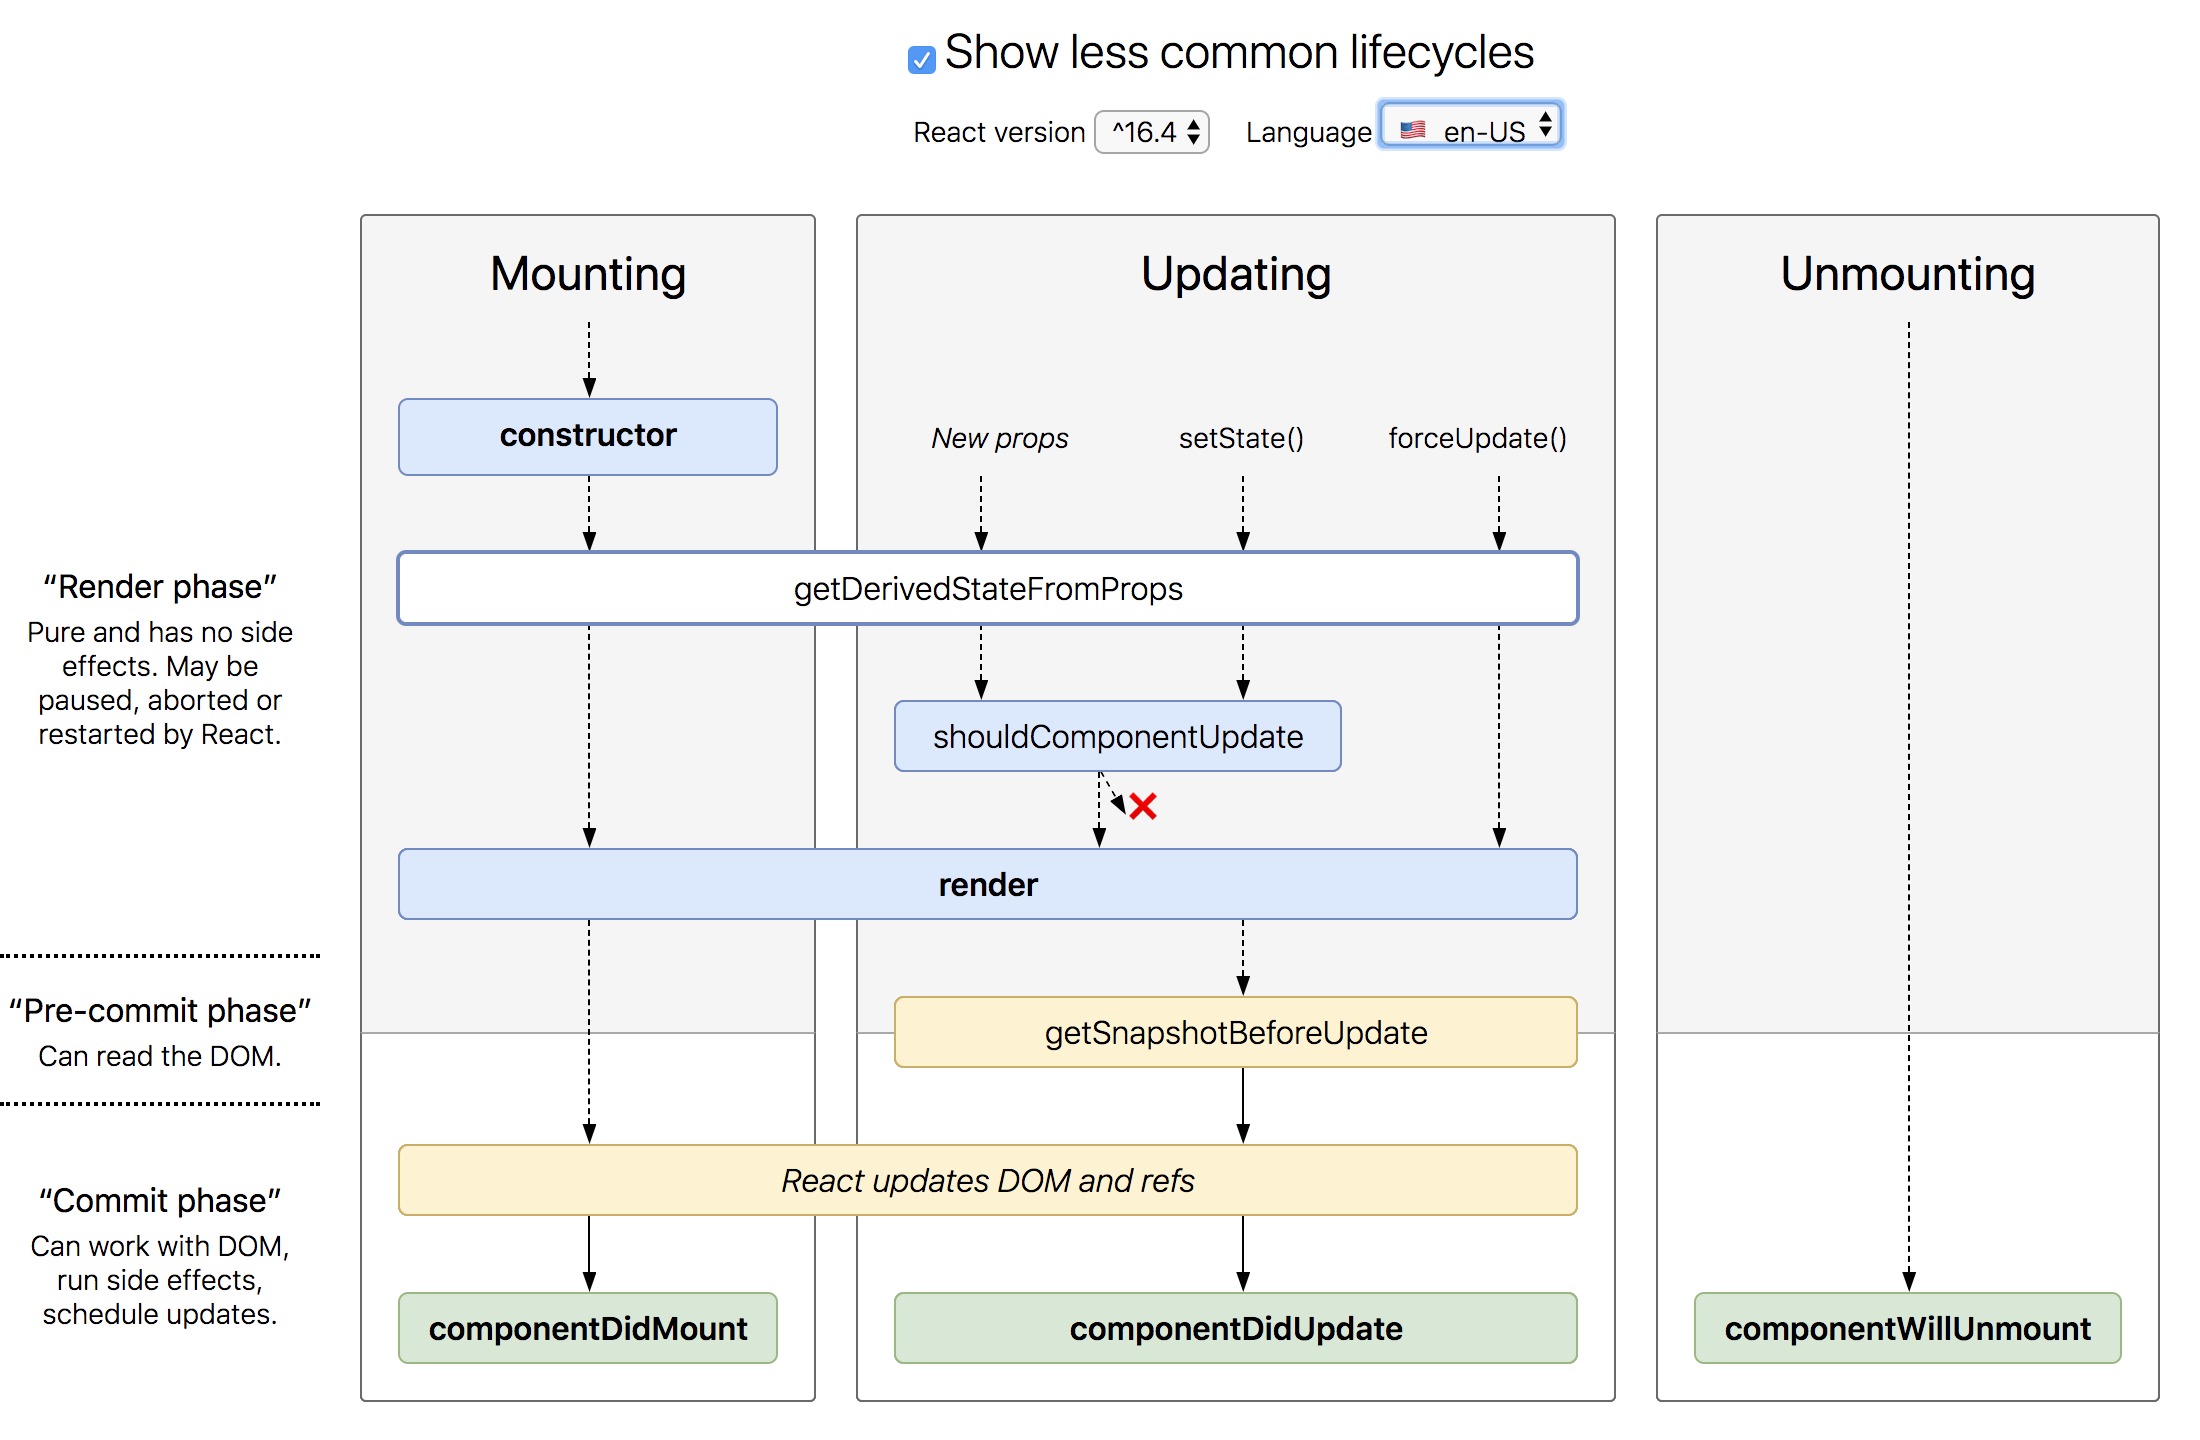
\includegraphics[width=\linewidth]{./img/React_lifecycle_methods.png}
    \caption{Dit diagram stelt een visuele referentie voor van de lifecycle methodes van een React component. Screenshot genomen op http://projects.wojtekmaj.pl/react-lifecycle-methods-diagram/}
    \label{fig:react-lifecycle-diagram}
\end{figure}

In applicaties met vele componenten is het vaak belangrijk om resources zo snel mogelijk vrij te maken die door de componenten werden ingenomen als ze verwijderd worden. Er bestaan enkele speciale methodes binnen de component klasse die code uitvoeren wanneer de component gekoppeld of ontkoppeld wordt. Deze methodes worden \texttt{lifecycle methods} genoemd. Raadpleeg \ref{fig:react-lifecycle-diagram} voor een visuele referentie. \autocite{React2019c}

\paragraph{render()}

De \texttt{render()} functie is de enige verplichte methode in een klasse component. Wanneer het opgeroepen wordt, moet het \texttt{this.props} of \texttt{this.state} overlopen en een van volgende types teruggeven: \autocite{React2019d}
\begin{itemize}
    \item React elementen
    \item Arrays en fragmenten
    \item Portals
    \item Strings en numbers
    \item Booleans of null
\end{itemize}

De render functie zou puur moeten zijn, het mag de state van een component niet aanpassen. Elke keer dat het opgeroepen wordt, moet het hetzelfde resultaat retourneren en het heeft geen directe interactie met de browser. Wanneer er toch interactie met de browser moet zijn, kan er gebruik gemaakt worden van andere lifecycle methodes. \texttt{render()} zal niet uitgevoerd worden wanneer \texttt{shouldComponentUpdate()} \texttt{false} retourneert. \autocite{React2019d}

\paragraph{constructor()}

Wanneer geen state geïnitialiseerd wordt en methodes niet gebonden worden, is er geen nood aan een contructor functie binnen de React component. De constructor van een component wordt aangeroepen voordat het gekoppeld wordt. Bij het implementeren van een constructor in een \texttt{React.component} subklasse moet \texttt{super(props)} opgeroepen worden als eerste statement. Als dat niet gebeurt, is \texttt{this.props} \texttt{undefined} en dat kan tot enkele rare bugs leiden. \autocite{React2019d}

In React bestaan constructor functies voor twee redenen. Als eerste om lokale state te initialiseren door een object toe te kennen aan \texttt{this.state}. Als tweede om event handler methodes te koppelen aan instanties. Binnen \texttt{constructor()} zou de call \texttt{setState()} nooit gebruikt mogen worden. In plaats daarvan kan de state direct geïnitialiseerd worden in de constructor. Dit is de enige plaats waar \texttt{this.state} direct toegewezen zou mogen worden. In alle andere methodes moet \texttt{this.setState()} gebruikt moeten worden. \autocite{React2019d}

\paragraph{componentDidMount()} 

Deze methode wordt opgeroepen direct nadat het gekoppeld werd. Alle initialisatie betreffende DOM nodes zou in \texttt{componentDidMount()} moeten komen. Als er data moet geladen worden vanuit een backend, dan is dit een goede plaats om een netwerk request te instantiëren. Het is wel belangrijk om deze subscriptions te sluiten in \texttt{componentWillUnmount()}. \autocite{React2019d}

In \texttt{componentDidMount()} kan de functie \texttt{setState()} direct gebruikt worden. Alhoewel dit voor een extra weergave zorgt, zal de gebruiker hiervan niets zien omdat dit gebeurt voordat de browser het scherm zal updaten. Dit is echter niet altijd aan te raden omdat dit vaak voor prestatieproblemen zorgt. In de meeste gevallen kan de initiële state in \texttt{constructor()} geïnitialiseerd worden, maar soms is het nodig om een DOM node af te meten voordat iets weergegeven wordt wanneer dit afhangt van de grote of plaats van de node. \autocite{React2019d}

\paragraph{componentDidUpdate()}

\texttt{componentDidUpdate()} is aangeroepen direct nadat een update voorgekomen is. Deze methode wordt niet uitgevoerd na de initiële weergave. Deze methode zou gebruikt moeten worden om aan het DOM te werken nadat er een update gebeurd is. Het is ook een goede plaats om hierin netwerkverzoeken te doen zolang de huidige props met de vorige vergeleken worden. Een netwerk request is mogelijks niet nodig wanneer de props niet aangepast zijn. \autocite{React2019d}

Binnen de methode kan \texttt{setState()} opgeroepen worden, maar het moet gewrapt worden in een conditie. Wanneer dit niet gebeurt, zal dit een oneindige loop veroorzaken. \texttt{componentDidUpdate()} zal ook niet uitgevoerd worden wanneer \texttt{shouldComponentUpdate()} \texttt{false} teruggeeft.  \autocite{React2019d}

\paragraph{componentWillUnmount()}

Deze methode wordt aangeroepen onmiddellijk voordat een component ontkoppeld en vernietigd zal worden. Alle nodige clean-up zoals het annuleren van netwerk request en het opruimen van subscriptions zou in deze methode uitgevoerd moeten worden.  \autocite{React2019d}

\texttt{setState()} zou nooit mogen opgeroepen worden in \texttt{componentWillUnmount()} omdat de component nooit meer opnieuw weergegeven zal worden. Eens een component losgekoppeld wordt, kan het nooit meer terug gekoppeld worden.  \autocite{React2019d}

\paragraph{Zelden gebruikte lifecycle methodes}

Volgende methodes kunnen in ongewone gevallen voorkomen. Ze kunnen soms handig zijn, maar in de meeste gevallen zijn ze niet nodig.  \autocite{React2019d}

\begin{itemize}
    \item shouldComponentUpdate()
    \item static getDerivedStateFromProps()
    \item static getDerivedStateFromProps()
    \item Error boundaries
    \item static getDerivedStateFromError()
    \item componentDidCatch()
\end{itemize}

\subsubsection{State correct gebruiken}

\paragraph{Wijzig state niet rechtstreeks}

Wanneer state rechtstreeks aangepast wordt, zal de component niet opnieuw weergegeven worden. In plaats daarvan moet de methode \texttt{setState()} gebruikt worden. De enige plaats waar state direct toegewezen kan worden is in de constructor. \autocite{React2019d}

\paragraph{State updates kunnen asynchroon zijn}

React kan meerdere \texttt{setState()} calls groeperen in een enkele update voor een betere prestatie. Omdat \texttt{this.props} en \texttt{this.state} asynchroon geüpdatet kunnen worden, is het niet aangeraden om te vertrouwen op die waarden om de volgende state te berekenen. Om te voorkomen dat de verkeerde waarden gebruikt worden in een \texttt{setState()} berekening, kan een tweede vorm van \texttt{setState()} gebruikt worden. Deze vorm verwacht een functie in plaats van een object. De functie ontvangt de vorige staat als eerste argument en de props van wanneer de update uitgevoerd wordt als tweede argument. \autocite{React2019d} %example?

\paragraph{State updates zijn samengevoegd}

Wanneer \texttt{setState()} aangeroepen wordt, zal React het meegegeven object samenvoegen met de bestaande state. Het samenvoegen is ondiep, dit betekent dat wanneer slechts een state attribuut moet veranderen, dan zal React enkel dat attribuut in de state aanpassen en de rest onaangetast laten. \autocite{React2019d} %example?

\subsubsection{De data vloeit naar beneden}

Zowel parent als kind kunnen niet weten of een bepaalde component stateful of stateless is en het zou ze niet mogen schelen of het gedefinieerd is als klasse of als functie. Daarom wordt state vaak lokaal of ingekapseld genoemd. Het is niet toegankelijk voor alle componenten dan degene die het bezit en kan aanpassen. Het is mogelijk voor een component om zijn state als props mee te geven aan child componenten. Dit wordt een \texttt{top-down} of een \texttt{unidirectionele} gegevensstroom genoemd. Een state is eigendom van een specifieke component en alle data of UI's die afgeleid zijn van die state kan enkel invloed hebben op componenten onder hen in de DOM tree. \autocite{React2019d}

\subsection{Events afhandelen}

Events afhandelen met React elementen is gelijkaardig aan het afhandelen van events in DOM elementen. Er zijn echter enkele verschillen in syntax. In de naamgeving van React events wordt gebruik gemaakt van \texttt{camelCase} in plaats van alles in \texttt{lowercase}. Daarnaast wordt met JSX een functie meegegeven als event handler in plaats van een string. Een ander verschil is dat men in React geen \texttt{false} kan retourneren om een event niet te laten doorgaan. Daarvoor moet expliciet de \texttt{preventDefault} methode gebruikt worden.  \autocite{React2019f}

Met React zou normaal gezien geen \texttt{addEventListener} opgeroepen moeten worden om listeners toe te voegen op een DOM element. In plaats daarvan kan gewoon een listener voorzien worden bij de initiële weergave.  \autocite{React2019f}

De betekenis van \texttt{this} is in JSX callbacks belangrijk. Net zoals in JavaScript zijn klasse methodes standaard niet gebonden. Wanneer een niet-gebonden methode meegegeven wordt aan een event handler, zal \texttt{this} in de callback \texttt{undefined} zijn. Dit is niet door React, maar door hoe JavaScript werkt. In het algemeen moeten methodes gebonden worden wanneer naar de methode gerefereerd wordt zonder haakjes. Binden gebeurt op de volgende manier: \texttt{this.method1 = this.method1.bind(this)}.  \autocite{React2019f}

Als de class field syntax niet gebruikt wordt, kunnen ook \texttt{arrow functions} gehanteerd worden in de callback. Het probleem met die syntax is dat er telkens de component weergegeven wordt, er een nieuwe callback wordt gemaakt. In de meeste gevallen is dit geen probleem, maar als de callback meegegeven wordt aan een child component, dan moet die component een extra weergave doen. Daarom is het aangeraden om binding te doen in de constructor of class field syntax te gebruiken om dit soort prestatieverlies te voorkomen. \autocite{React2019f}

\subsubsection{Argumenten meegeven aan event handlers}

Binnen een loop is het niet ongewoon om een extra parameter te willen meegeven aan een event handler. In een \texttt{arrow function} moeten de argumenten expliciet meegegeven worden, terwijl met een \texttt{bind} worden alle argumenten automatisch doorgestuurd. \autocite{React2019f}

\subsection{Conditionele weergave}

In React kunnen afzonderlijke componenten gemaakt worden die het gedrag bevatten die de applicatie exact nodig heeft. Daarna kunnen enkele weergegeven worden, afhankelijk van de staat van de applicatie. Conditioneel weergeven werkt in React op dezelfde manier als condities werken in JavaScript. Door JavaScript operatoren zoals \texttt{if} of de \texttt{conditionele operator} toe te passen, kunnen elementen gecreëerd worden die de huidige staat van de applicatie voorstellen waarop React de UI zal updaten. \autocite{React2019g}

\subsubsection{Elementen als variabelen}

In React kunnen elementen opgeslagen worden in variabelen. Dit kan helpen om een deel van een component conditioneel weer te geven zonder dat de rest van de output gewijzigd wordt. Gebaseerd op de huidige staat kunnen dan bepaalde delen getoond worden.  \autocite{React2019g}

Terwijl een variabele declareren en een \texttt{if} statement gebruiken een goede manier is om een component conditioneel weer te geven, is het soms beter om een kortere syntax te hanteren. In JSX zijn er bepaalde manieren om dit inline te doen. \autocite{React2019g}

\subsubsection{Inline 'if' met de logische '\&\&' operator}

In JSX kan gelijk welke expressie geïntegreerd worden door ze te wrappen in accolades. Dit geldt ook voor de logische \texttt{\&\&} operator van JavaScript. Dit kan handig zijn om conditioneel een element toe te voegen. Dit werkt omdat JavaScript enkel en alleen maar de tweede expressie in een \texttt{\&\&} operator zal evalueren wanneer de eerste \texttt{true} is. Als de eerste expressie \texttt{true} is, zal het element net na de \texttt{\&\&} in de output verschijnen, maar wanneer de eerste expressie \texttt{false} is, dan zal het element genegeerd worden en dus niet verschijnen. \autocite{React2019g}

\subsubsection{Inline 'if-else' met de conditionele operator}

Een andere manier om elementen conditioneel weer te geven, is door de conditionele operator \texttt{conditie ? true : false} van JavaScript te gebruiken. Deze manier kan gebruikt worden voor grotere expressies, maar in dat geval wordt het vaak minder leesbaar. Net als in JavaScript is het aan de developer om een gepaste stijl te kiezen die leesbaar is voor zichzelf en eventueel het team. Wanneer een conditie te ingewikkeld wordt, is het misschien handig om componenten te extraheren zoals besproken in \ref{componenten extraheren}. \autocite{React2019g}

\subsubsection{Voorkomen dat componenten weergegeven worden}

In heel uitzonderlijke gevallen is het gewenst om component te verbergen, ook al werd het weergegeven door een andere component. Dit kan door \texttt{null} te retourneren in plaats van zijn render output. \texttt{Null} retourneren in de render methode van een component beïnvloedt niets in de levenscyclus van die component. Alle lifecycle methodes zullen nog steeds aangeroepen worden. \autocite{React2019g}

\subsection{Lijsten en sleutels}

In JavaScript kan een lijst getransformeerd worden de \texttt{map()} functie toe te passen. De functie overloopt alle elementen in de lijst, waarop dan een behandeling wordt toegepast. De functie op zich retourneert een nieuwe lijst. In React kan een array getransformeerd worden in een lijst van elementen op ongeveer dezelfde manier. \autocite{React2019h}

\subsubsection{Meerdere componenten weergeven}

In React kunnen collecties van elementen gecreëerd worden en in JSX opgenomen worden door accolades te gebruiken. Door elk element in een array te mappen naar een DOM object en het resultaat op te slaan in een variabele, kunnen meerdere componenten weergegeven worden door enkel het resultaat weer te geven. \autocite{React2019h}

\subsubsection{Een basische lijst component}

Lijsten worden bij voorkeur weergegeven in een component. Echter wanneer een component een array binnenkrijgt via \texttt{props}, wordt er een waarschuwing gegenereerd dat een \texttt{key} moet voorzien worden voor de items in de lijst. Een \texttt{key} / \texttt{sleutel} is een speciaal string attribuut moet opgenomen worden bij het maken van lijsten.  \autocite{React2019h}

\subsubsection{Sleutels}

\texttt{Sleutels} zijn een attribuut die React helpen om bij te houden welke items gewijzigd, toegevoegd of verwijderd werden. Elk element in een array zou een \texttt{key} moeten krijgen om het een stabiele identiteit te geven. De beste manier om een \texttt{key} te kiezen is om een string te gebruiken die een uniek item uit de lijst identificeert onder de andere items uit die lijst. In de meeste gevallen wordt het ID-attribuut gebruikt. Als er geen unieke ID's zijn, kan de index van het item gebruikt worden, maar best als laatste redmiddel. Indexen als \texttt{keys} gebruiken kan enkel en alleen maar als de volgorde van de items niet verandert. Anders kan dit effect hebben op de prestaties en negatieve gevolgen voor de state van de component. Wanneer geen expliciete \texttt{key} wordt voorzien, zal React standaard de index gebruiken.  \autocite{React2019h}

\subsubsection{Sleutels moeten enkel uniek zijn binnen de array}

Sleutels die gebruikt worden binnen een array moeten enkel uniek zijn in die array. Ze moeten dus niet globaal uniek zijn. Dezelfde sleutels kunnen gebruikt worden voor verschillende arrays. Sleutels worden enkel gebruikt als hint voor React. Ze worden niet doorgegeven aan componenten. Als een component die waarde toch nodig heeft, kan die als een prop worden doorgegeven onder een andere naam. \autocite{React2019h}

\subsubsection{Map() insluiten in JSX}

JSX staat toe om gelijk welke expressie in te sluiten in accolades. Dit omvat dus ook het resultaat van een \texttt{map()} functie. Soms kan dit resulteren in code die beter leesbaar is, maar deze stijl kan ook misbruikt worden. Wanneer de body van de \texttt{map()} functie te genest wordt, dan is het waarschijnlijk een goed idee om de component te extraheren zoals besproken in \ref{componenten extraheren}. \autocite{React2019h}

\subsection{Formulieren}

Form elementen in HTML werken iets anders dan andere DOM elementen in React, omdat form elementen standaard een interne state bijhouden. Wanneer een standaard HTML formulier ingediend wordt, dan zal de gebruiker naar een nieuwe pagina geleid worden. In de meeste gevallen is dit niet de gewenste functionaliteit. Meestal is het handig om een JavaScript functie te hebben die het indienen van de form behandelt en daarbij toegang heeft tot de inhoud van de form die door de gebruiker werd ingevuld. De standaard manier om dit te bereiken in React is aan de hand van een techniek die \texttt{gecontroleerde componenten} wordt genoemd. \autocite{React2019i}

\subsubsection{Gecontroleerde componenten}

In HTML onderhouden elementen zoals \texttt{<input>}, \texttt{<textarea>} en \texttt{<select>} vaak hun eigen state en updaten het volgens de input van de user. In React wordt veranderlijke state bijgehouden door een property in de component. Beide manieren kunnen gecombineerd worden door de state in React de enige bron van waarheid te maken. De component die de form weergeeft, beheert ook wat er gebeurt wanneer de gebruiker iets wijzigt in de form. Een form element waarvan de waarde van de input op deze manier gecontroleerd wordt door React wordt een \texttt{gecontroleerde component} genoemd. \autocite{React2019i}

Wanneer de \texttt{setState()} wordt uitgevoerd na de \texttt{onChange()} event, kan de state van de React component beschouwd worden als de enige bron van waarheid. Met een \texttt{gecontroleerde component} heeft elke verandering een bijhorende handlerfunctie. Dit maakt het gemakkelijk om de input van gebruikers aan te passen of te valideren.  \autocite{React2019i}

\subsubsection{De textarea tag}

In HTML wordt een \texttt{<textarea>} tag gedefinieerd door zijn kinderen. Echter, in React wordt een \texttt{value} attribuut gebruikt in plaats. Op deze manier kan een form die gebruik maakt van een \texttt{<textarea>} geschreven worden op een gelijkaardige manier als een \texttt{<input>} tag. \autocite{React2019i}

\subsubsection{De select tag}

In HTML zal een \texttt{<select>} tag een \texttt{drop down} lijst genereren. De items binnen deze lijst zijn alle \texttt{<option>} children binnen de \texttt{<select>} tag. Een initieel item kan geselecteerd worden door aan de \texttt{<option>} het \texttt{selected} attribuut te vermelden. In plaats van dergelijk attribuut te gebruiken, hanteert React een \texttt{value} attribuut op de root \texttt{<select>}. Voor een \texttt{gecontroleerde component} veel handiger omdat het maar een enkel item moet updaten. \autocite{React2019i}

\subsubsection{De file input tag}

In HTML kan een gebruiker met behulp van \texttt{<input type=''file'' />} een of meerdere files vanuit hun opslag uploaden naar een server of laten manipuleren door JavaScript via de \texttt{file API}. Omdat deze \texttt{value} \texttt{read-only} is, wordt dergelijk component in React een \texttt{uncontrolled component} genoemd. \autocite{React2019i}

\subsubsection{Meerdere inputs behandelen}

Bij het behandelen van meerdere input elementen in een form kan een \texttt{name} attribuut aan elk element toegevoegd worden, waarna een handler functie beslist wat te doen gebaseerd op de \texttt{event.target.name}. \autocite{React2019i}

\subsubsection{Alternatieven voor gecontroleerde componenten}

Soms kan het wel veel werk zijn om gecontroleerde componenten te maken, omdat voor elke manier waarop data aangepast kan worden een event handler geschreven moet worden en alle state moet door een React component gesluisd worden. Dit kan vooral vervelend worden wanneer een bestaande applicatie omgezet moet worden naar een React applicatie. In deze situatie is het misschien handig om gebruik te maken van \texttt{ongecontroleerde componenten}.  \autocite{React2019i}

\subsection{State naar boven verheffen}

Vaak moeten meerdere componenten dezelfde veranderlijke state afspiegelen. In dat geval wordt aangeraden om de state te verheffen naar de dichtste gelijke voorouder. Dit wordt \texttt{lifting state up} genoemd. De lokale state wordt verplaatst naar een voorouder en van daaruit doorgegeven en aangepast. De voorouder wordt dan de \texttt{bron van waarheid}. Aangezien alle componenten die data nodig heeft van deze bron een (klein)kind is van die component, zal de data altijd in sync zijn.  \autocite{React2019j}

In een React applicatie zou er voor elke data die verandert slechts een \texttt{bron van waarheid} mogen zijn. Normaal gezien wordt state eerst toegevoegd aan de component die het nodig heeft om weergegeven te worden. Daarna kan het, als andere componenten het ook nodig hebben, naar boven verheven worden naar de dichtstbijzijnde gemeenschappelijke voorouder. In plaats van state te proberen synchroniseren, zou vertrouwd moeten worden op een \texttt{top-down data flow}. \autocite{React2019j}

Het verheffen van state houdt in dat er meer code geschreven moet worden, maar als voordeel heeft het dat het minder werk zal inhouden om bugs te vinden en isoleren. Omdat state zich maar in slechts een enkele component bevindt, zijn de locatiemogelijkheden van de bug veel kleiner geworden.  \autocite{React2019j}

\subsection{Compositie versus overerving}

React heeft een krachtig compositiemodel en raadt aan om compositie te gebruiken om code tussen componenten opnieuw te gebruiken in plaats van overerving. Bij het gebruik van overerving komen vaak problemen voor die opgelost kunnen worden met compositie. \autocite{React2019k}

\subsubsection{Insluiting}

Sommige componenten weten nog niet op voorhand wat hun kinderen zullen zijn. Bij zulke componenten is het aangeraden om de speciale \texttt{children} prop te gebruiken om de children direct in hun output te plaatsen. Op die manier kunnen andere componenten willekeurige children meegeven aan die component door ze te nesten in JSX. \autocite{React2019k}

\subsubsection{Specialisatie}

In sommige gevallen kunnen bepaalde componenten gezien worden als een speciaal geval van een generieke component. Zo kan bijvoorbeeld een \texttt{WelcomeDialog} een speciale \texttt{Dialog} component zijn. In React wordt dit ook bereikt via compositie, waar een specifieke component een meer generieke component weergeeft en het configureert met props.  \autocite{React2019k}

\subsubsection{Wat met overerving?}

Bij Facebook gebruiken ze React met duizenden componenten en ze hebben, naar eigen zeggen, nog geen enkele use case tegengekomen waarbij ze overerving zouden aanraden. Props en compositie geven de nodige flexibiliteit om het uiterlijk en gedrag van een component aan te passen. \autocite{React2019k}

 

\section{Mithril.js}

Mithril is een modern client-side framework, gemaakt voor het bouwen van single page applications. %uitleggen
Het is klein in download, snel in performance en voorziet routing en XHR-tools. \autocite{Mithril2019c}

Dit framework is vergelijkbaar met React, maar het is eenvoudiger en meer capabel. Mithril vervangt de behoefte aan bibliotheken zoals jQuery. De kleine bestandsgrootte en gemakkelijke API zorgt ervoor dat Mithril ideaal is om geïntegreerde JavaScript-widgets of user interfaces die hoge performance vereisten hebben, te maken. \autocite{Gilbert2018}

Mithril was oorspronkelijk geschreven door Leo Horie. Het framework werd uitgebreid en verbeterd tot wat het tegenwoordig is dankzij het werk van de community. \autocite{Mithril2019b}

\subsection{Virtuele DOM nodes}
\subsubsection{Virtueel DOM}

Een virtuele DOM-structuur is een JavaScript-datastructuur die een \texttt{DOM tree} beschrijft. Het bestaat uit een aantal geneste virtuele DOM nodes, genaamd \texttt{vnodes} \autocite{Mithril2019g}

Meestal worden virtuele DOM's opnieuw opgebouwd bij een rendercyclus. Deze cyclus vindt plaats na een event of na data changes. Bij zo'n rendercyclus bekijkt Mithril de vorige versie van de vnode-structuur en wijzigt enkel de DOM-elementen op plaatsen waar een aanpassing plaatsvond. Nieuwe vnodes maken is goedkoper dan het wijzigen van de DOM. \autocite{Mithril2019g}

\subsubsection{Basis}

Vnodes zijn JavaScript objecten die delen van het DOM voorstellen. De virtuele DOM-machine van Mithril verbruikt de vnodes-structuur en stelt een DOM-structuur op. Vnodes kunnen aangemaakt worden aan de hand van het \texttt{m()} hyperschrift. Hyperschrift kan ook \texttt{componenten} verbruiken. \autocite{Mithril2019g}

\subsubsection{Structuur}

Vnodes zijn JavaScript objecten die een element voorstellen. Ze kunnen volgende eigenschappen hebben:

\begin{table}[!htbp]
    \begin{tabular}{p{0.15\textwidth} p{0.85\textwidth}}
        tag      & De \texttt{nodeName} van een DOM element. De tag kan ook een string zijn als de vnode een fragment, een text-node of vertrouwd HTML node is.                                                                                     \\
        key      & De waarde die gebruikt wordt om een DOM element te mappen naar zijn respectievelijke item in een array van data.                                                                                                                 \\
        attrs    & Een hashmap van DOM attributen, events, eigenschappen en lifecycle methodes.                                                                                                                                                     \\
        children & Een array van de kinderen van de vnode. Meestal zijn dit ook vnodes, maar in sommige gevallen kan dit een string, een number of een boolean zijn.                                                                                \\
        text     & Dit wordt enkel gebruikt als een vnode enkel een text node heeft als kind. Dit wordt enkel gedaan om performance redenen.\footnote{Component vnodes gebruiken deze property niet ook al hebben ze enkel een text-node als kind.} \\
        dom      & Verwijst naar het element dat correspondeert met de vnode.                                                                                                                                                                       \\
        domSize  & Deze eigenschap wordt enkel gebruikt in fragmenten en vertrouwde HTML nodes. Het stelt het aantal DOM elementen voor die de vnode vertegenwoordigt. \\
        state & Een object dat voorzien wordt door de \texttt{core engine} en bewaard wordt doorheen cyclussen. Bij een POJO component vnode erft het state object de eigenschappen van de component klasse/object over. \\
        events & Een object dat de event handlers opslaat zodat deze later verwijderd kunnen worden door gebruik te maken van de DOM API. Net zoals het state-object wordt deze ook bewaard doorheen de rendercyclussen. Deze eigenschap wordt intern gebruikt door Mithril en zou nooit gebruikt of aangepast mogen worden. \\
        instance & Een object voor componenten. Het is een opslaglocatie voor de waarde die de view methode teruggeeft. Deze eigenschap wordt ook intern gebruikt door Mithril en zou nooit gebruikt of aangepast mogen worden. \\
    \end{tabular}
\end{table} \autocite{Mithril2019g}

\subsubsection{Soorten vnodes}

In Mithril bestaan er 5 verschillende soorten vnodes. Deze wordt bepaald door de \texttt{tag} attribuut. 

\begin{table}[!htbp]
    \begin{tabular}{p{0.15\textwidth} p{0.85\textwidth}}
        Element & Vertegenwoordigt een DOM element. \\
        Fragment & Vertegenwoordigt een lijst van DOM elementen waarvan de parent ook andere DOM elementen kan bevatten die zicht niet in de lijst bevinden. \\
        Text & Vertegenwoordigt een DOM text-node \\
        Trusted HTML & Vertegenwoordigt een lijst van DOM elementen van een HTML string \\
        Component & Vertegenwoordigt het DOM dat gegenereerd wordt bij het weergeven van de component. Dit kan enkel als de \texttt{tag} een component is die een \texttt{view} methode bevat.
    \end{tabular}
\end{table}
\autocite{Mithril2019g}

In een virtuele DOM structuur moet alles een vnode zijn, dus ook text. De \texttt{m()} utility normaliseert zijn \texttt{children} argument en verandert tekst in text vnodes en geneste arrays in fragment vnodes. Het eerste argument van de \texttt{m()} functie kan enkel een element tag naam of een component zijn. Trusted HTML vnodes kunnen gemaakt worden aan de hand van de methode \texttt{m.trust()} \autocite{Mithril2019g}

\subsubsection{Monomorfe klasse}

De \texttt{mithril/render/vnode} wordt gebruikt door Mithril om alle vnodes aan te maken. Dit zorgt ervoor dat moderne JavaScript machines optimaal virtuele DOM structuren kunnen vergelijken door altijd vnodes te compileren met deze ene verborgen klasse. \autocite{Mithril2019g}

\subsubsection{Anti-patterns vermijden}

Vnodes vertegenwoordigen de staat van het DOM op een gegeven tijdstip. De rendermachine van Mithril gaat ervan uit dat een vnode die opnieuw gebruikt wordt onaangepast is. Het aanpassen van een vnode die gebruikt werd in een vorige weergave zal resulteren in een \texttt{undefined} gedrag. \autocite{Mithril2019g}

Het is mogelijk om vnodes te hergebruiken om een render cycle te vermijden, maar het is beter om gebruik te maken van de \texttt{onbeforeupdate} hook te gebruiken.  \autocite{Mithril2019g}

\subsection{Componenten}
\subsubsection{Structuur}

Componenten zijn een mechanisme die gebruikt worden om delen van de view in te kapselen. Hierdoor wordt de code gemakkelijker om te structureren of om opnieuw te gebruiken. Elk JavaScript object dat een \texttt{view} methode heeft is een Mithril component. Deze componenten kunnen gebruikt worden door gebruik te maken van de \texttt{m()} functie. \autocite{Mithril2019a}

\subsubsection{Lifecycle methodes}

Componenten hebben dezelfde lifecycle methodes als vnodes. Bij elke lifecycle methode wordt een \texttt{vnode} als argument meegegeven, net zoals bij de \texttt{view} methode. Zoals de andere types vnodes kunnen componenten extra lifecycle methodes hebben wanneer ze gebruikt worden als vnode type. \autocite{Mithril2019a}

Lifecycle methodes in vnodes overschrijven de component methodes niet, ook niet omgekeerd. De lifecycle methodes van componenten worden altijd opgeroepen na de methodes van de vnode. Dezelfde naam kiezen voor callback functies als de lifecycle methode namen zou dus altijd vermeden moeten worden. \autocite{Mithril2019a}

\subsubsection{Data meegeven aan componenten}

Om data mee te geven aan componenten kan door een \texttt{attrs} object mee te geven als tweede parameter in de hyperschrift functie. %m(ExampleComponent, {name: `Floyd`})
Deze data kan worden geraadpleegd in de view van de component of in de lifecycle methodes via \texttt{vnode.attrs} \autocite{Mithril2019a}
%var ExampleComponent = {view: function(vnode) {return m('div', 'hello, ' + vnode.attrs.name)}} 

\subsubsection{State}

Zoals alle virtuele DOM nodes kunnen component vnodes een state hebben. Op deze manier kunnen zaken als objectgeoriënteerde structuren, inkapseling en separation of concerns  ondersteund worden. \autocite{Mithril2019a}

Een component aanpassen zorgt niet voor een DOM update. Dit gebeurt wanneer een event handler getriggerd wordt, wanneer een HTTP request (gemaakt via \texttt{m.request}) vervuld is of wanneer de browser navigeert naar een andere route. Om een redraw geforceerd te laten doorgaan kan gebruik gemaakt worden van \texttt{m.redraw()}. \autocite{Mithril2019a}

\paragraph{Closure component state}

Het is mogelijk om component state te gebruiken bij POJO componenten, maar dat is in het algemeen niet de beste aanpak. Een betere manier is door gebruik te maken van een closure component. Dat is simpelweg een wrapper functie die een POJO component instantie retourneert die op zich zijn eigen closed-over scope meedraagt. \autocite{Mithril2019a}

Met deze closure componenten kan state bewaard worden door variabelen die gedeclareerd staan in de buitenste functie. Ook functies die in de closure component gedeclareerd staan hebben toegang tot de state variabelen. \autocite{Mithril2019a}

Deze closure componenten worden op dezelfde manier gebruikt als POJO componenten. Het voordeel hiervan is dat er geen gebruik gemaakt moet worden van \texttt{this}. \autocite{Mithril2019a}

\paragraph{POJO component state}

Het is altijd aangeraden om closure componenten te gebruiken wanneer state moet bijgehouden worden. Er kan echter toch state bijgehouden worden in POJO componenten en die kan dan op drie manieren opgevraagd worden, namelijk als blueprint bij initialisatie, via \texttt{vnode.state} of via het \texttt{this} keyword in component methodes. \autocite{Mithril2019a}

\subsubsection{Klassen}

Componenten kunnen ook geschreven worden aan de hand van het \texttt{class} sleutelwoord. Deze class componenten moeten een \texttt{view()} methode definiëren. Deze methode wordt gedetecteerd via \texttt{.prototype.view} om in de DOM structuur weergegeven te worden. Ook klasse componenten worden op dezelfde manier gebruikt als normale componenten. Ook in klasse componenten kan state bijgehouden worden en deze kan beheerd worden door zijn attributen en methodes. State wordt aangeroepen via het \texttt{this} sleutelwoord, maar om de juiste referentie te verkrijgen moeten arrow functions gebruikt worden voor de event handler callbacks. \autocite{Mithril2019a}

\subsubsection{Gemixte soorten componenten}

Componenten kunnen gelijk welke soort component als kind hebben. Er zijn geen restricties op de soort kinderen qua component. \autocite{Mithril2019a}

\subsubsection{Speciale attributen}

Mithril gebruikt enkele property keys. Het is aangeraden om deze te vermijden in/als attributen van normale componenten. Deze keys zijn \autocite{Mithril2019a}
\begin{itemize}
    \item Lifecycle methodes, nl. \texttt{oninit}, \texttt{oncreate}, \texttt{onbeforeupdate}, \texttt{onupdate}, \texttt{onbeforeremove} en \texttt{onremove}
    \item \texttt{key}
    \item \texttt{tag}
\end{itemize}

\subsubsection{Anti-patterns vermijden}

Hoewel Mithril heel flexibel is, is het toch afgeraden om bepaalde patterns te vermijden. \autocite{Mithril2019a}

\paragraph{'Fat' componenten vermijden}

In het algemeen is een `fat` component een component met eigen instance methodes. Functies in \texttt{vnode.state} of in \texttt{this} zijn af te raden omdat deze niet hergebruikt kan worden in andere componenten. Het is ook eenvoudiger om de code te refactoren wanneer deze in de data laag staat in plaats van in state. Code die hergebruikt moet worden, wordt best in een module geplaatst. \autocite{Mithril2019a}

\paragraph{vnode.attrs niet meegeven andere componenten}

Om de interface flexibel te maken en een simpele implementatie te garanderen lijkt het logisch om alle attributen (\texttt{vnode.attrs}) door te geven aan de child componenten. In plaats daarvan zouden slechts enkele attributen meegegeven mogen worden aan child componenten. \autocite{Mithril2019a}

\paragraph{Vermijd het maken van component definities in views}

Als er een component gecreëerd wordt binnen een view functie, dan zal elke redraw een andere clone hebben van de component. Dit betekent dat componenten die dynamisch aangemaakt werden via een factory  ook altijd opnieuw van nul worden aangemaakt. \autocite{Mithril2019a}

\paragraph{Vermijd het maken van component instanties buiten views}

Als een component instantie buiten een view functie gemaakt wordt, dan zullen toekomstige redraws de vnode vergelijken, maar omdat deze dezelfde referentie krijgt, zal deze vnode overgeslagen worden en er zal geen update gebeuren.  \autocite{Mithril2019a}

\subsection{Lifecycle methodes}

\subsubsection{Gebruik}

Componenten en vnodes kunnen allemaal lifecycle methodes hebben, ook \texttt{hooks} genoemd. Deze methodes worden opgeroepen op verschillende tijdstippen tijdens het bestaan van een DOM element. \autocite{Mithril2019e}

Alle lifecycle methodes krijgen de vnode als eerste argument. Het \texttt{this} keyword in de callback van de methodes wordt gekoppeld aan de \texttt{vnode.state}. Hooks kunnen enkel aangeroepen worden als gevolg van de \texttt{m.render()} call. Ze worden niet aangeroepen als het DOM aangepast wordt zonder Mithril. \autocite{Mithril2019e}

\subsubsection{De levenscyclus van een DOM element}

Een DOM element wordt meestal gecreëerd en aan het document toegevoegd. Daarna kunnen zijn attributen of children geüpdatet worden wanneer een UI event getriggerd wordt. Het kan ook verwijderd worden van het document. \autocite{Mithril2019e}

Wanneer een element verwijderd wordt, kan het tijdelijk opgeslagen worden in een \texttt{memory pool}. Elementen in deze pool kunnen hergebruikt worden in een volgende update. Dat proces heet \texttt{DOM recycling}. Door het recycleren van een bestaand element kunnen de prestatiekosten van het maken van een nieuw element vermeden worden. \autocite{Mithril2019e}

\paragraph{Oninit}

De \texttt{oninit(vnode)} hook wordt aangeroepen voordat een vnode behandeld wordt door de virtuele DOM machine. Deze hook wordt gegarandeerd uitgevoerd voordat zijn DOM element vastgemaakt wordt aan het document en voordat zijn kinderen uitgevoerd worden. In de oninit(vnode) hook zou de \texttt{vnode.dom} nooit opgeroepen mogen worden. Deze methode wordt niet aangeroepen wanneer een element geüpdatet wordt, maar wel wanneer een verwijderd element gerecycleerd wordt uit de memory pool. De oninit hook is vooral nuttig voor het initialiseren van component state aan de hand van de argumenten die meegegeven werden met \texttt{vnode.attrs} of \texttt{vnode.children}. \autocite{Mithril2019e}

\paragraph{Oncreate}

De \texttt{oncreate(vnode)} hook wordt aangeroepen nadat een DOM element gecreëerd is en toegevoegd is aan het document. Deze lifecycle methode wordt gegarandeerd uitgevoerd op het einde van de render cyclus. Net zoals oninit wordt deze hook ook niet aangeroepen wanneer een element geüpdatet wordt. Echter, anders dan oninit kunnen elementen waarvan de vnodes een oncreate hook hebben niet gerecycleerd worden. De oncreate hook is handig voor het lezen van lay-out waarden die een redraw kunnen veroorzaken, voor het starten van animaties en voor het initialiseren van derde partij bibliotheken die een referentie nodig hebben naar het DOM element. \autocite{Mithril2019e}

\paragraph{Onupdate}

De \texttt{onupdate(vnode)} hook wordt aangeroepen nadat een DOM element geüpdatet werd terwijl het aan het document verbonden is. De methode wordt gegarandeerd uitgevoerd op het einde van de render cyclus. Deze hook wordt enkel aangeroepen als het element al bestond in de vorige render cyclus. Het wordt nooit aangeroepen wanneer het element gecreëerd of gerecycleerd wordt. DOM elementen waarvan zijn vnodes een onupdate hook hebben kunnen niet gerecycleerd worden. De onupdate hook is vooral handig voor het lezen van lay-out waarden die een redraw kunnen veroorzaken en voor het dynamisch aanpassen van state in derde partij bibliotheken die de UI\footnote{User Interface} aanpassen, nadat model data gewijzigd is. \autocite{Mithril2019e}

\paragraph{Onbeforeremove}

De \texttt{onbeforeremove(vnode)} hook wordt aangeroepen voordat een DOM element van het document losgekoppeld wordt. Wanneer een promise geretourneerd wordt, zal Mithril het element slechts loskoppelen wanneer de promise voldaan is. Deze hook wordt enkel aangeroepen op de elementen die hun \texttt{parentNode} verliezen, maar het wordt niet aangeroepen in zijn kinderen. Ook hier worden elementen waarvan de vnodes een onbeforeremove hook bevatten, niet gerecycleerd. \autocite{Mithril2019e}

\paragraph{Onremove}

De \texttt{onremove(vnode)} hook wordt aangeroepen voordat een DOM element verwijderd wordt van het document. Deze methode wordt uitgevoerd op elk element dat uit het document verwijderd wordt, ongeacht of het rechtstreeks van de parent werd losgemaakt of dat het een child is van een ander element dat werd losgemaakt. De onremove hook is nuttig voor het runnen van opkuis taken. \autocite{Mithril2019e}

\paragraph{Onbeforeupdate}

De \texttt{onbeforeupdate(vnode, old)} hook wordt aangeroepen voordat een vnode vergeleken wordt in een update. Als deze functie false retourneert, dan voorkomt Mithril dat in deze vnode een aanpassing gebeurt, waardoor ook de kinderen niet aangepast worden. Deze hook is handig voor het verminderen van de vertraging tijdens updates. \autocite{Mithril2019e}

\subsection{Keys}

Keys zijn een mechanisme die toelaten om DOM elementen te herschikken in een NodeList. Een key wordt gebruikt om DOM element te verbinden met een dataobject aan de hand van het id van dat object. Het key property zou altijd het unieke id-attribuut van objecten binnen een array moeten zijn. \autocite{Mithril2019d}

\subsubsection{Gebruik}

Een veelgebruikt patroon is om data te hebben die bestaat uit een array van objecten, hiervan wordt dan een lijst van vnodes gegenereerd die elk object in de array mappen. \autocite{Mithril2019d}

Het probleem hierbij ligt bij het aanpassen van die array. Stel dat uit een array van twee objecten het eerste item werd weggehaald, dan weet Mithril niet of het eerste object werd verwijderd of het tweede werd verwijderd en het eerste aangepast werd. Dit kan voor problemen zorgen bij het focussen van elementen of wanneer er stateful jQuery plug-ins worden gebruikt, kunnen deze een foutieve interne state hebben na de update. \autocite{Mithril2019d}

Wanneer een lijst van vnodes afkomstig is uit een dynamische array van data is het beter om een \texttt{key} property toe te voegen aan elke vnode. Dit zorgt ervoor dat Mithril op een slimme manier het DOM kan herschikken zodat elk DOM element juist gemapt blijft aan zijn respectievelijke item in de data array. \autocite{Mithril2019d}

\subsubsection{Single-child keyed fragmenten}

Soms is het nodig om een component op bevel opnieuw te initialiseren. Hiervoor kan het patroon van een \texttt{single-child keyed fragment} gebruikt worden, waarbij de key aangepast wordt om het element te verwijderen en opnieuw te initialiseren. \autocite{Mithril2019d}

Het kan ook gebonden worden aan een gekende identiteit, bijvoorbeeld wanneer een backend wordt aangesproken om een item op te halen aan de hand van een id. Wanneer het id in de routing wordt gebruikt, kan de key gekoppeld worden aan \texttt{m.route.params('id')}. Wanneer de user niet meer naar die ene item wil kijken, zal de key veranderen, waardoor het element verwijderd zal worden van het document. \autocite{Mithril2019d}

\subsubsection{Key gerelateerde problemen debuggen}

Keys kunnen soms tot verwarrende problemen leiden wanneer het verkeerd gebruikt wordt. Een typisch symptoom is dat de applicatie state corrupt blijkt te zijn geworden na enkele gebruiker interactie, meestal wanneer data verwijderd wordt.  \autocite{Mithril2019d}

\paragraph{Vermijd wrapper elementen rond keyed elementen}

Keys moeten geplaats worden op de vnode dat een direct kind is van de array. Dat betekent dat wanneer een element gewrapt wordt in een div element, de key eigenlijk in het div element moet geplaats worden. \autocite{Mithril2019d}

\paragraph{Vermijd het verbergen van keys in component root elementen}

Wanneer de code gerefactored wordt en een component gemaakt wordt, dan moet de key verdwijnen uit de component. In de m utility functie moet de key dan geplaatst worden op de component zelf. \autocite{Mithril2019d}

\paragraph{Vermijd het wrappen van keyed elementen in arrays}

Arrays zijn vnodes en daarvoor ook keyable. Keyed elementen zouden nooit gewrapt mogen worden in arrays buiten single-child keyed fragmenten. \autocite{Mithril2019d}

\paragraph{Vermijd variabele types}

Keys moeten altijd van het type string zijn. Als ze dat niet zijn, worden ze gecast naar een string. Om dezelfde keys te vermijden (bijvoorbeeld string `1` en number 1 zou in dezelfde key resulteren) zou maar een type gebruikt mogen worden. \autocite{Mithril2019d}

\paragraph{Vermijd het gebruik van keyed en niet-keyed vnodes in dezelfde array}

Een array van vnodes kan enkel keyed vnodes of niet-keyed vnodes bevatten, niet beide. Wanneer dit toch gebeurt, zal er een error optreden. \texttt{null}, \texttt{undefined} of booleans worden beschouwd als niet-keyed vnodes. \autocite{Mithril2019d}

\paragraph{Vermijd het doorgeven van model data direct naar de component wanneer het model key gebruikt als data property}

Het is mogelijk dat er een \texttt{key} attribuut nodig is in het data model. Dit kan voor problemen zorgen in combinatie met Mithril's \texttt{key} logica. Om problemen te voorkomen zou de data gewrapt moeten worden zodat Mithril deze niet beschouwt als render instructies. \autocite{Mithril2019d}

% voorbeeld?

\subsection{Het auto-redraw systeem}

Mithril implementeert een virtueel DOM vergelijkingssysteem om snel te kunnen weergeven. Daarbij biedt het ook meerdere mechanismes om gedetailleerde controle te krijgen over de weergave van een applicatie. \autocite{Mithril2019f}

Het auto-redraw systeem van Mithril synchroniseert het DOM wanneer er aanpassingen gemaakt zijn in de data laag. Het systeem wordt ingeschakeld wanneer \texttt{m.mount} of \texttt{m.route} aangeroepen wordt, maar blijft uitgeschakeld als de applicatie uitsluitend gebootstrapt wordt door \texttt{m.render} calls. Wanneer er toch een redraw zou moeten gebeuren, kan deze manueel getriggerd worden door gebruik te maken van \texttt{m.redraw()}. Deze methode zal een asynchrone redraw starten. \autocite{Mithril2019f}

Het auto-redraw systeem bestaat simpelweg uit een re-render functie die wordt uitgevoerd op de achtergrond als bepaalde functies voltooid zijn. \autocite{Mithril2019f}

\subsubsection{Na event handlers}

Mithril zal automatisch een redraw laten doorgaan na DOM event handlers die gedefinieerd staan in een Mithril view. Deze redraw kan manueel uitgeschakeld worden door gebruik te maken van de instelling \texttt{e.redraw} op \texttt{false} te zetten.  \autocite{Mithril2019f}

\subsubsection{Na m.request}

Mithril zal ook automatisch een redraw laten doorgaan wanneer een \texttt{m.request} voltooid wordt. De redraw kan gedeactiveerd worden door een extra object toe te voegen aan de request, waarbij het object een \texttt{background} property heeft die op true staat. \autocite{Mithril2019f}

% example

\subsubsection{Na een verandering in route}

Ook na een \texttt{m.route.set()} call en na een routewijziging via links (door gebruik te maken van \texttt{m.route.Links}) zal Mithril een redraw laten doorgaan. \autocite{Mithril2019f}


% meer hier!!

% subsection Hooks
% subsection Suspence
% subsection Concurrent Mode